\documentclass[conference]{IEEEtran}

\usepackage{amsmath}   % For advanced math symbols
\usepackage{graphicx}  % For including images
\usepackage{cite}      % For handling citations
\usepackage[hidelinks=true]{hyperref}  % For hyperlinks
\usepackage{lipsum}    % For example/filler text

% All separate paragraphs in italics in the document below act as commentary to explain where content came from or stuff that still needs to be done. This MUST be all deleted before submission

% *** TITLE AND AUTHOR ***
\title{Electronically Switching TIA Design \\
    \large ENGR302 Final Project Report - 2024}

\author{
    \IEEEauthorblockN{Evgeny Zhilkin, Louis Smith, Mario Pankusz, Max Mawby}
    \IEEEauthorblockA{
        Electrical \& Electronics Engineering \\
        Te Herenga Waka - Victoria University of Wellington \\
        Wellington, Aotearoa New Zealand \\
    }
}

\begin{document}

\maketitle

% *** ABSTRACT ***
\begin{abstract}

The Measurement Standards Laboratory of New Zealand (MSL) need a transimpedence amplifier whose gain can be switched remotely, to streamline the process of measuring low level currents from photodiodes. This project aimed to solve their problem by building a TIA with electronic switches that are controlled by a microcontroller, allowing a user to select gain via a USB cable. \\
\textit{Still needs to include evaluation/results of the project.}\\

\end{abstract}

% *** INTRODUCTION ***
\section{Introduction}

\textit{Still needs: a summary of the evaluation section, basically the outcome or "findings" of the project.} \\

The New Zealand Measurement Standards Laboratory (NZMSL) plays a crucial role in ensuring the accuracy of measurement standards in New Zealand. One of their key responsibilities is the precise measurement of light levels from different sources, which is fundamental for applications ranging from environmental monitoring to industrial quality control. Accurate light measurement is vital for maintaining consistency in standards and ensuring that industries can rely on these measurements for their processes. In order to maintain accuracy, anytime the testing room is exposed to light there is down time to ensure light levels return to the baseline. NZMSL would like to reduce this down time, by reducing the number of times a person has to physically enter the room during a testing session. The goal of this project was to design a system that can be controlled remotely to solve this issue. \\

The current setup at NZMSL involves manual gain control on their transimpedence amplifier (TIA) that they use to measure small photodiode currents. Manually switching gain requires entering the experiment room , resulting in a loss of time as the room must darken again. This project involves designing a solution that enables remote gain switching without exposing the experiment to light, significantly reducing the downtime and allowing gain adjustments without interrupting the experimental environment.
Since NZMSL conducts experiments across a wide range of photodiodes, the solution must perform effectively within an operating current range from nano amps (nA) to milliamps (mA). Given NZMSL's role as a standard for measurements, it is crucial to ensure the solution's accuracy. This requires minimising interference with the input signal and carefully selecting components to reduce noise and inaccuracies in the amplification and switching circuits. \\

The remainder of this report will delve into: documented examples of TIA designs that were used to inform the outcomes of this project, the design and its various parts, implementation of the design, evaluation of the final design, final remarks and what could be done in the future to improve the design.

% *** MAIN BODY ***
\section{Related Work}

\textit{This section should provide a comprehensive overview of existing research and literature relevant to the topic, demonstrating your understanding of the field.} \\

Texas Instruments have published an in-depth exploration of designing transimpedance amplifiers (TIAs) for applications requiring the amplification of extremely low currents (such as nA) \cite{hashemi_2015}. The TIA is crucial in converting this tiny input current into a corresponding output voltage, making it suitable for this application which demands precise current measurement and control. To achieve a 0-10V output range, the amplifier design must carefully consider the feedback resistor, as its value directly determines the voltage output for a given input current. For an input current of nanoamps, the feedback resistor would need to be in the range of M$$\Omega$$. Additionally, selecting an operational amplifier with ultra-low input bias current and low noise characteristics is essential to maintain signal integrity and accuracy at such low current levels. The document emphasises the importance of ensuring stability and managing bandwidth limitations, which are critical when dealing with high gain configurations in TIA circuits.

Another document from Texas Instruments \cite{Texas_Instruments} gives a detailed guide on designing a photodiode amplifier using an operational amplifier configured as a trans-impedance amplifier. It is designed to amplify a light-dependent current from a photodiode resulting in an analogue voltage output. The document outlines key design considerations, such as selecting the appropriate gain resistor and feedback capacitor to meet desired bandwidth requirements which in this case is 0. The circuit is specifically designed with a 5V supply voltage, aiming to achieve a maximum output voltage of 4.9V with a minimum input current of 0A which in this application will need to be modified to allow for the 0V – 10V range required on the output. The design process is supported by detailed simulations and recommended component choices, particularly the OPA323 op amp, known for its low bias current and rail-to-rail output capabilities which may be required if using ground as the negative rail in this amplifier. This document serves as a comprehensive reference for designing photodiode amplifier circuits with robust performance in various applications.

An article \cite{black_brisebois_2014} by Black and Brisebois (Linear Technology) provides another view of an in-depth analysis of the requirements and challenges in designing transimpedance amplifiers for wide-range photodiodes, particularly in high-speed and high dynamic range applications. It discusses the critical role of low input bias current, low noise, and low input capacitance in achieving optimal TIA performance. The authors emphasise the importance of selecting amplifiers with FET input stages to minimise input current variation with temperature, as well as the need for careful board layout to reduce stray capacitances and leakage currents. Additionally, the consideration of adding a feedback capacitor is highlighted as a crucial step for ensuring circuit stability by compensating for input capacitance. The LTC6268 op amp is highlighted as a solution that meets these stringent requirements, offering femtoampere-level input bias current, high bandwidth, and low noise, making it ideal for advanced photodiode circuits. The discussion also underscores the trade-offs between gain, noise, and bandwidth in TIA design, illustrating the complexity of achieving stability and precision in such circuits.

In another article \cite{baker_2017}, Bonnie Baker delves into the task of designing transimpedance amplifiers for precision photo-sensing applications. Baker emphasises the importance of achieving the correct phase margin, which is required for determining the circuit’s step response, overshoot characteristics, and quality factor. The article outlines a systematic approach to TIA design, beginning with defining the operational amplifier's output swing and progressing to the calculation of the feedback resistor and capacitor, which are central to setting the desired phase margin. A detailed discussion on the calculation of key frequencies and the impact of feedback components on circuit stability and bandwidth highlights the delicate balance needed in TIA design. Additionally, Baker underscores the importance of selecting an amplifier with low input bias current and offset voltage, as well as the iterative process of fine-tuning the feedback capacitor to achieve a preferred phase margin. The article also considers the role of parasitic capacitances and the necessity of incorporating a feedback capacitor within the design to ensure stability. Through a practical example involving the Texas Instruments OPA192IDBVR and Vishay's TEMD6200FX01 photodiode, Baker illustrates the application of these design principles, providing engineers with valuable insights into the optimization of TIA circuits for precision opto-sensing.\\

The primary takeaway from these previous works is the importance in the specific op-amp selection. In particular for our purposes, a low input bias current and offset voltage are the most important factors. Because the input from NZMSL's photodiode will essentially be a DC current, there is little reason to be concerned with frequency response characteristic like bandwidth for this project. 

\textit{Copied from progress report, edited, still need to setup the references in this doc}

\section{Design}

\textit{The aim of this section is to articulate the technical solution with sufficient detail and clarity. When solving a complex problem, there are normally many different approaches one can take — each with its own advantages and disadvantages. It is expected that groups will initially consider a range of different solutions and narrow these down. The reasons why a particular approach was discounted should be documented here.} \\

At the most basic level there are three components or parts to the design. A microprocessor, switching circuit, and the transimpedance amplifier (TIA) circuit(s). Figure \ref{fig:1} illustrates the following process: a microprocessor controls the switching circuit which directs the path of the input current (from the client’s photodiode) through the TIA. This effectively gives the microcontroller the ability to set the gain of the system. \\

Figure \ref{fig:2} provides an alternative illustration of the fundamental workings of the design, including the basic arrangement of a TIA circuit. By changing the value of the feedback resistor between values on the order of $10^3$ to $10^9$, the TIA can output any current between 1nA to 1mA as a 1-10V voltage, satisfying requirements 1.1 and 2.1.

\begin{figure}
    \centering
    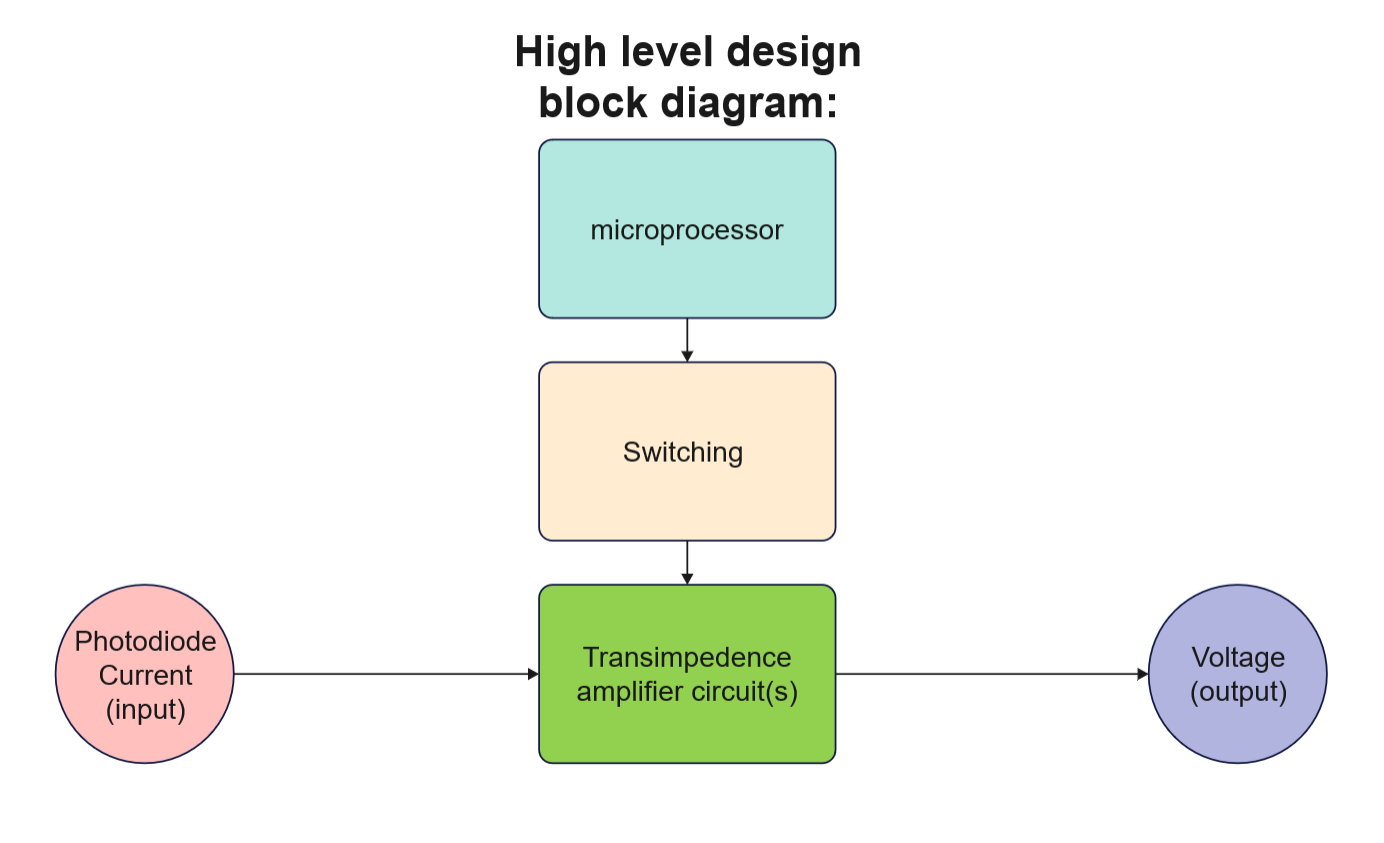
\includegraphics[width=0.8\linewidth]{ENGR302_TIA_blockl_diagram_v2.png}
    \caption{High level block diagram of the switching TIA design.}
    \label{fig:1}
\end{figure}

\begin{figure}
    \centering
    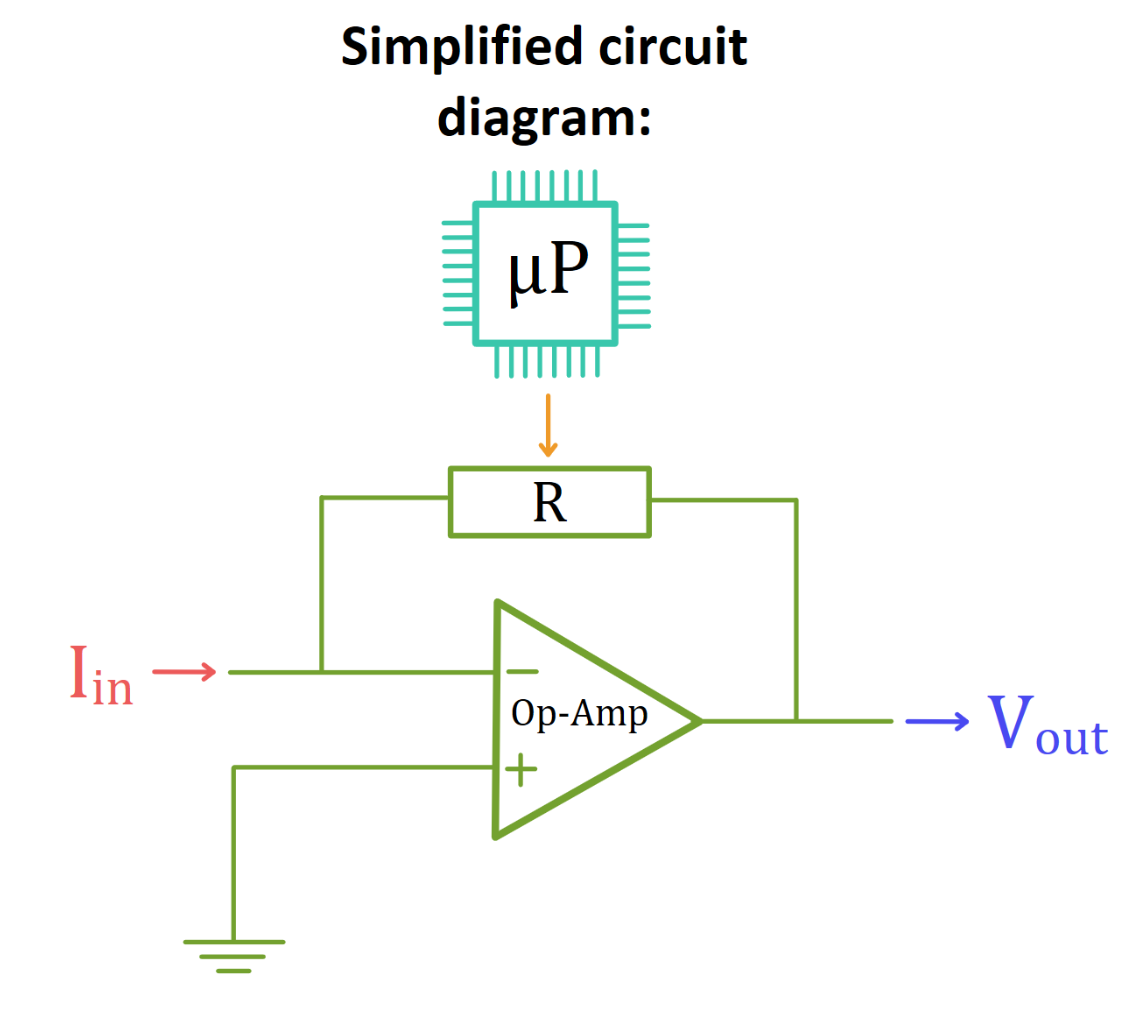
\includegraphics[width=0.8\linewidth]{Simplified_Circuit_Diagramv2.png}
    \caption{Simplified Circuit diagram of the switching TIA design}
    \label{fig:2}
\end{figure}

\subsection{Hardware topologies}

There are three TIA topologies that could be used for this design. This is a major consideration for the design, as the primary goal of the project is focused on the ability to change the gain of the TIA. \\

The first topology, in the top left corner of figure \ref{fig:3}, is the simplest and likely the most common. It puts feedback resistors in parallel with an op-amp, allowing switches to select which resistor, and therefore gain, is being used in the TIA circuit. NZMSL’s current TIAs use this topology with a manual dial physically switching out the resistors.
The other two topologies dedicate an individual op-amp for each level of gain. The benefit of this is it allows a specific op-amp with ideal characteristics to be selected for each gain value, instead of restricting the entire circuit to one op-amp which may behave optimally for some gain values, but not so for others. \\

The top right corner of figure \ref{fig:3} illustrates a series configuration of multiple op-amps. The first circuit would be the only transimpedance amplifier, all the rest would be regular non-inverting amplifiers as they no longer have to turn a current into a voltage, and would instead need to amplify the voltage from the last circuit to the next decade of gain. The switching in this case would only be on the output, and select which op-amps output to feed to the output of the system.  \\

\begin{figure}
    \centering
    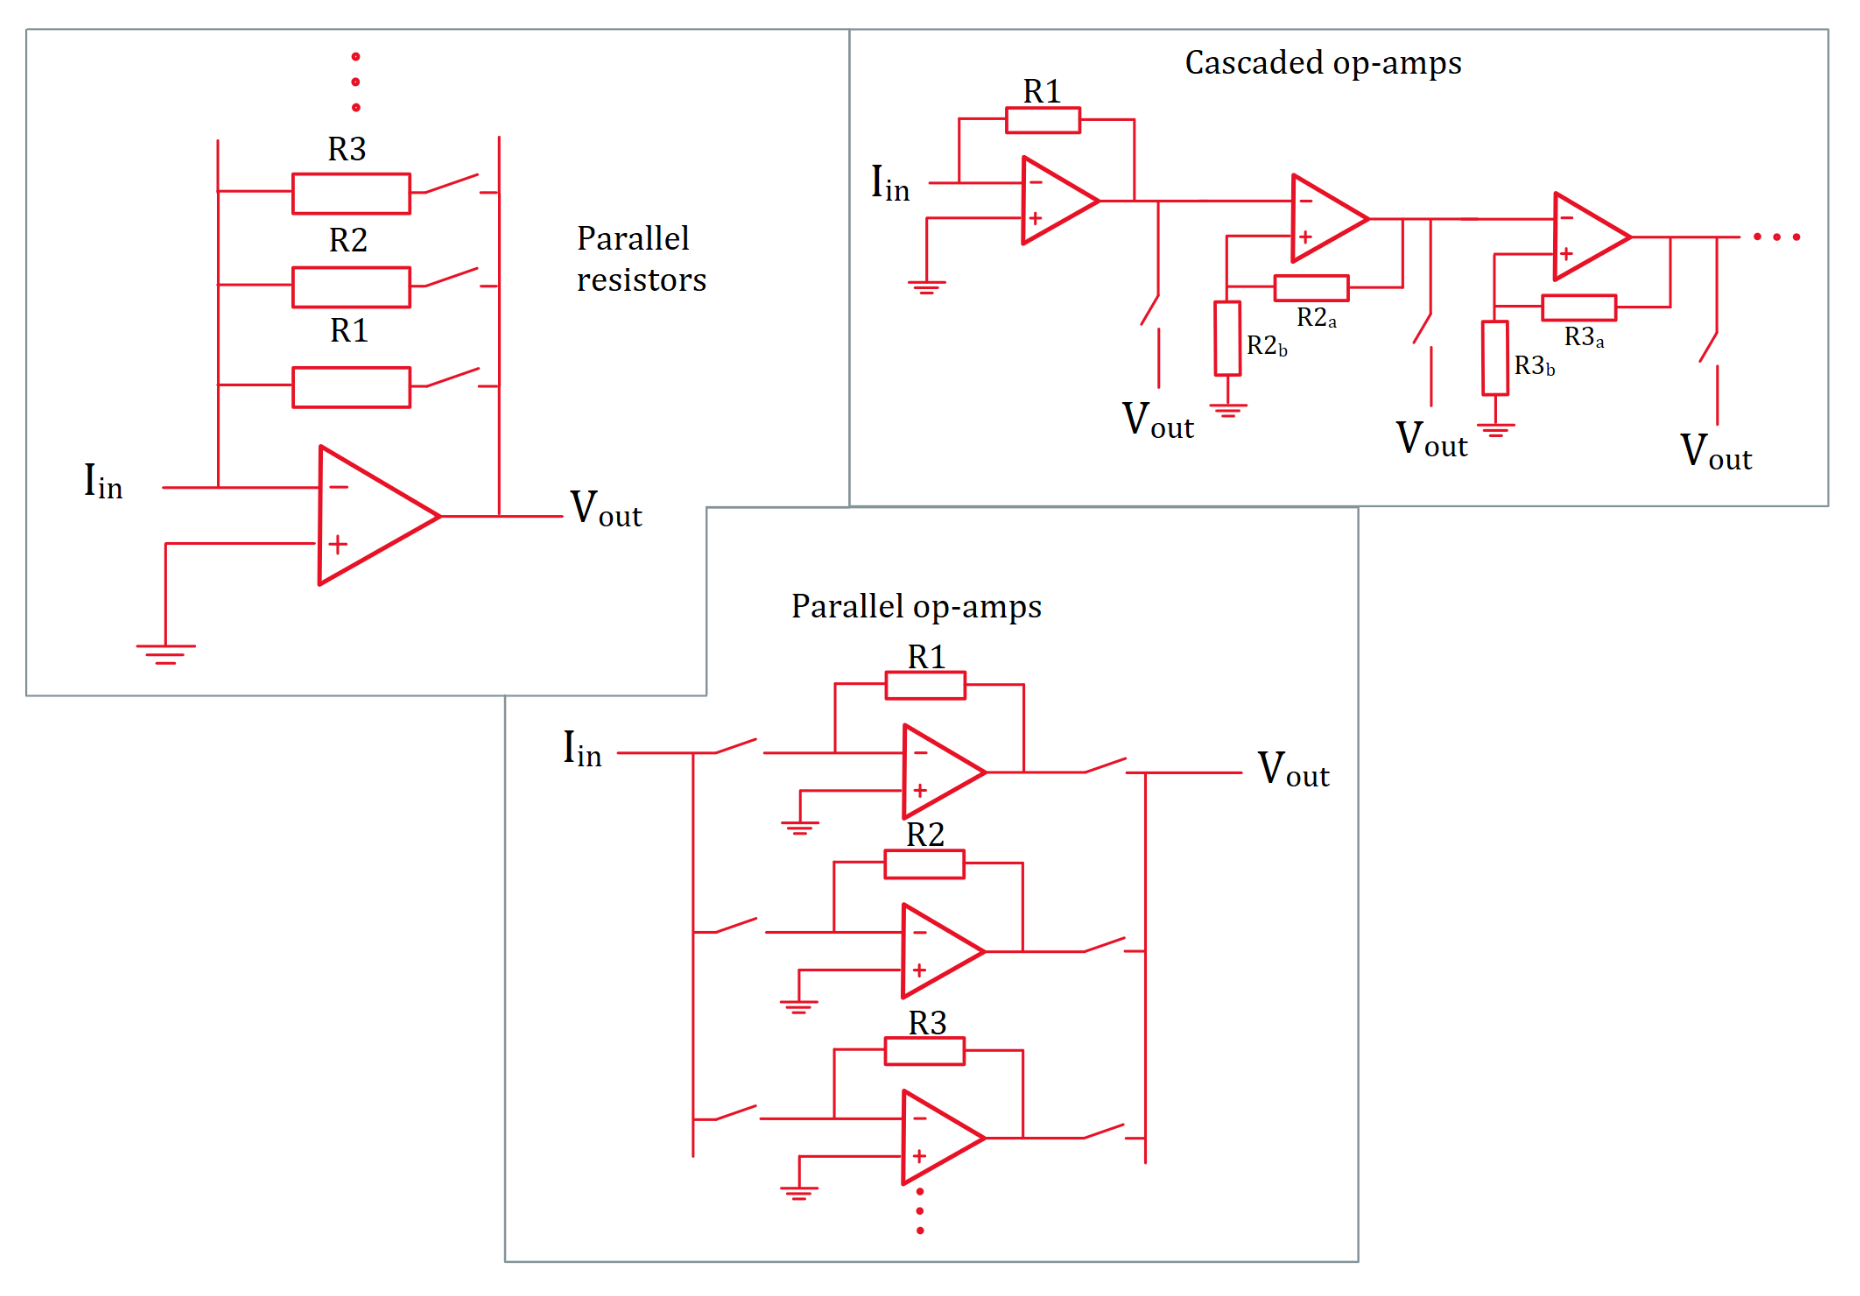
\includegraphics[width=0.8\linewidth]{TopologiesV3.png}
    \caption{Three possible TIA topologies.}
    \label{fig:3}
\end{figure}

The disadvantage of a set of TIA’s connected in series is that the first circuit will be a major limiting factor. If the first op-amp and feedback resistor receive a current that is beyond what they are designed to accurately amplify (whether it’s too low or high), it could distort the input and cascade that distortion all the way to the output, effectively nullifying the benefits of having multiple TIA circuits fine tuned to specific gain values. \\

The final design in figure \ref{fig:3} illustrates the chosen topology of this project. This design combines the benefits of both of the other topologies. It takes TIA circuits that have each been designed for a specific gain, and puts them in parallel to avoid unnecessarily modifying the input current, satisfying requirement R1.4. \\

\subsection{Switching considerations}

A factor which had to be taken into account before implementation was that of leakage current across switches. Leakage currents across switches have the potential to tamper with the input current of the circuit, with a small portion being leaked through open switches into disconnected portions of the circuit. This has the potential to add error to both the input and output, even with switches being employed on both sides of the TIA. This would degrade the input signal, while the output signal could receive leakage current from one or more of the inactive areas of the circuit. The possibility of the output being tampered with is reduced as any leakage current would need to first pass the input side switch, pass through the TIA and then also leak through the output side switch.
To eliminate the possibility of any leakage currents, Latching relays were used for switching. Latching relays are electromechanical switches that maintain their state without any power needing to be applied. By way of being a mechanical contact switch reduces the chance of there being almost any leakage currents through latching relays. Because of the way latching relays work, the control current and the switched current are electrically isolated, meaning the control current will not interfere with the current being measured. Both of these characteristics make latching relays ideal for this application.\\

\textit{This whole section needs to be replaced with an explanation of how our switching works, and what it does to mitigate any issues} \\

\subsection{Software/control design}

The control of the electronic switches is done through a BeagleBone Black micro-controller. The BeagleBone Black is an open-source development board based on the ARM Cortex-A8 processor \cite{beaglebone®_black}. While the processing capabilities of the BeagleBone are beyond what is necessary for this project, it was chose because of the availability and access to documentation, allowing for a good starting point for setting up a control/communication system between a user and the TIA's gain switches. 
Another advantage of the BeagleBone is that it runs a very fast version of Linux right away, which allows easy setup of a TCP server using C programs. The server facilitates real-time communication with a client to control the design, enabling the user to switch between multiple gain modes and query the current status remotely. The server communicates via TCP messages, receiving commands and responding while managing the hardware’s configuration settings.
Details of the server, and its interfacing with the beagleBone's output pins connected to the relays, will be elaborated on in the implementation section of this report.

\subsection{Power Supply}

As this is an active electronic design, it will need a power supply. Given that the output voltage needs to be able to reach 10V (as seen in requirement 2.1), the op-amps require at least 10V to power their rails. The BeagleBone however, needs 5V to be powered. The simplest solution is to power them separately with 12V and 5V power supplies. This is not the neatest or most user friendly approach, and could be replaced by using a single power supply with a DC-DC voltage converter in the system. However, neither neatness nor user-friendliness are high priorities in this design, therefore they are not necessary before end user implementation. \\

\section{Implementation}

\textit{The purpose of this section is for you to discuss how you transformed the technical solution (the design) to its realisation (the artifact). Similar to the Design section, you must provide clear and sufficient descriptions.} \\

\subsection{Schematic}

Figure \ref{fig:4} illustrates the full TIA Schematic, which implements the parallel configuration of six TIAs whose input and output is switched to select the desired gain. On the left is the main area of interest; six op-amps configured as TIAs, with the power input and control headers that will output to the BeagleBone beneath, a voltage reference on the right, and the BNC connectors above that. \\

In figure \ref{fig:5} can be seen the magnified schematic of a single TIA op-amp. Each one is largely the same as this. The output (pin 6) and the input (pin 3) of the opa-amp is connected through a latching relay to an output header. A decoupling capacitor sits between the power rails to reduce any noise from the power supply. And the all important gain resistor, which is the only varying component in each sub-circuit, connects the output and negative input, making it a transimpedence amplifier. 

\begin{figure}
    \centering
    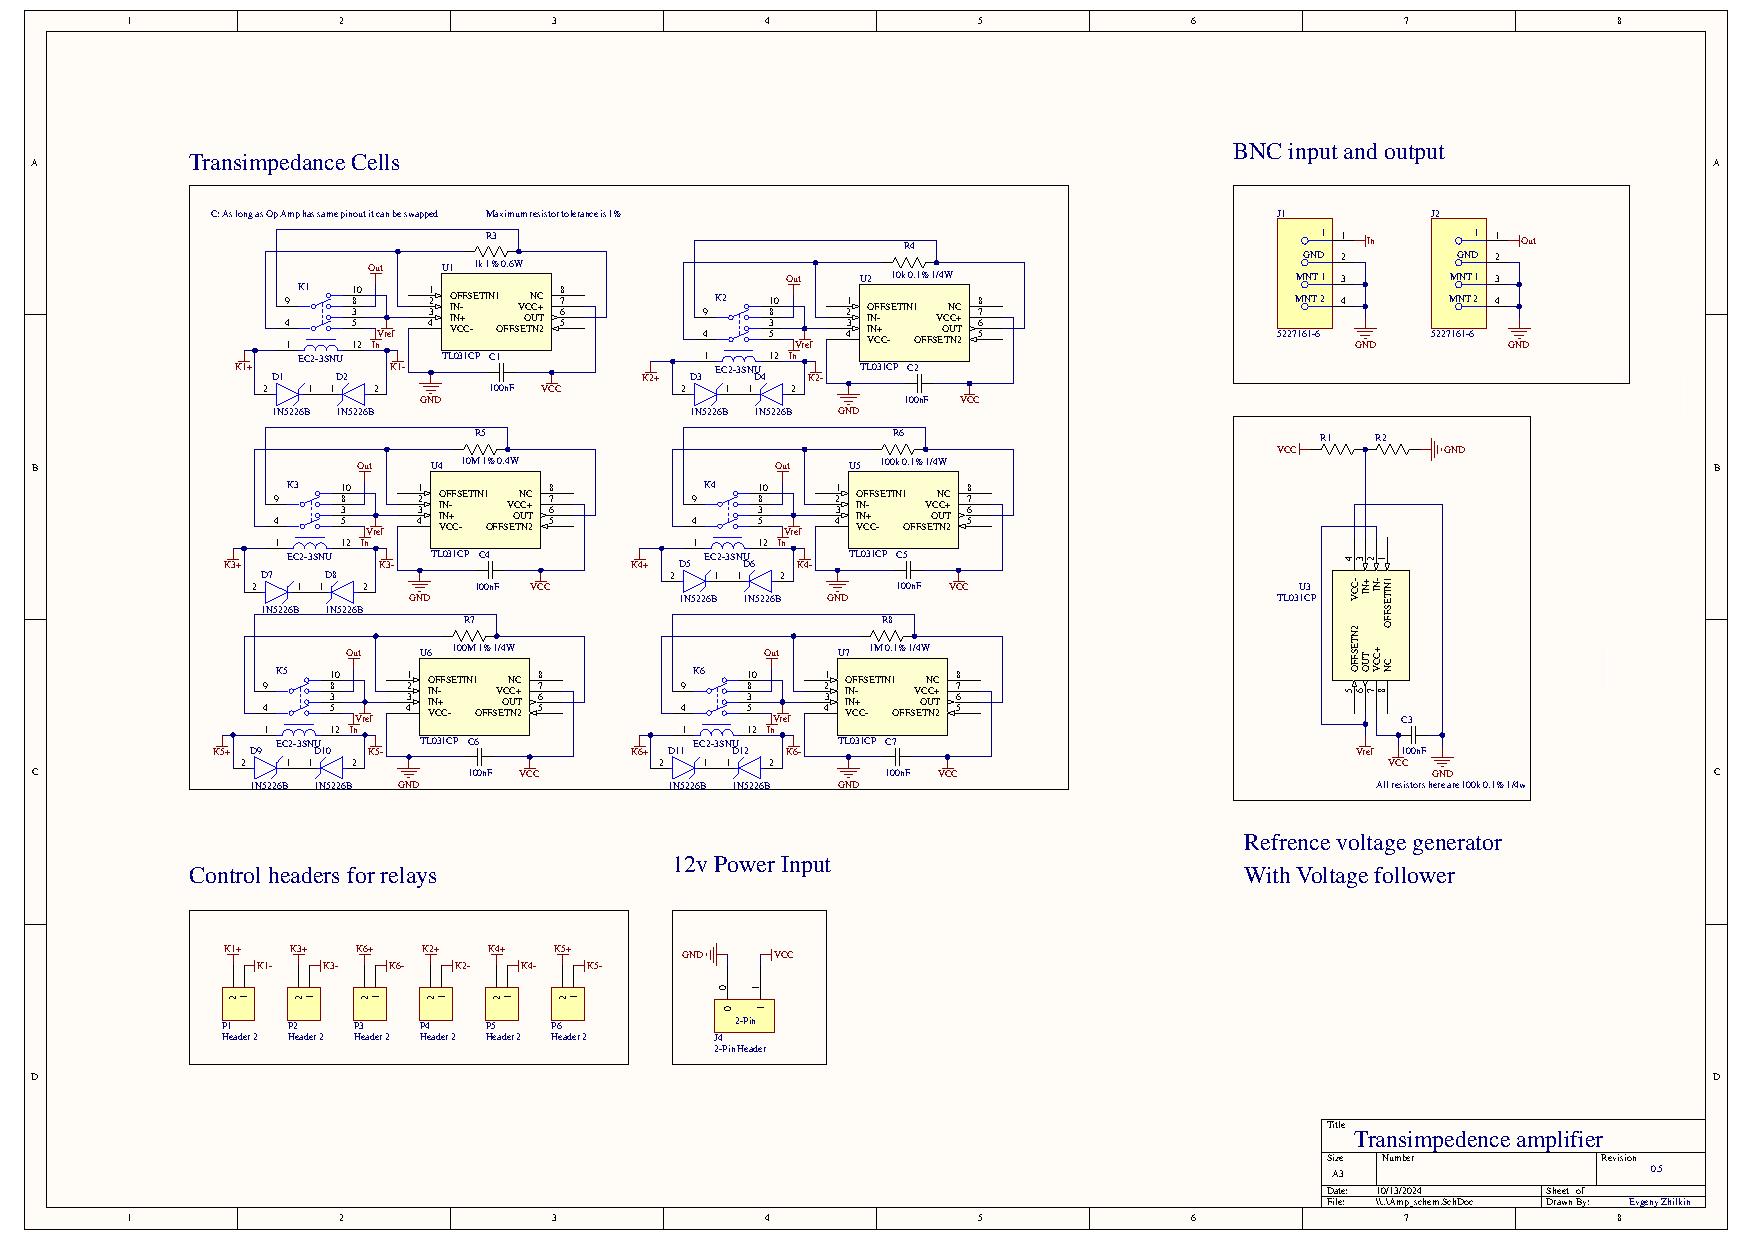
\includegraphics[width=\linewidth]{Amp_schem.pdf}
    \caption{Full TIA schematic}
    \label{fig:4}
\end{figure}


\begin{figure}
    \centering
    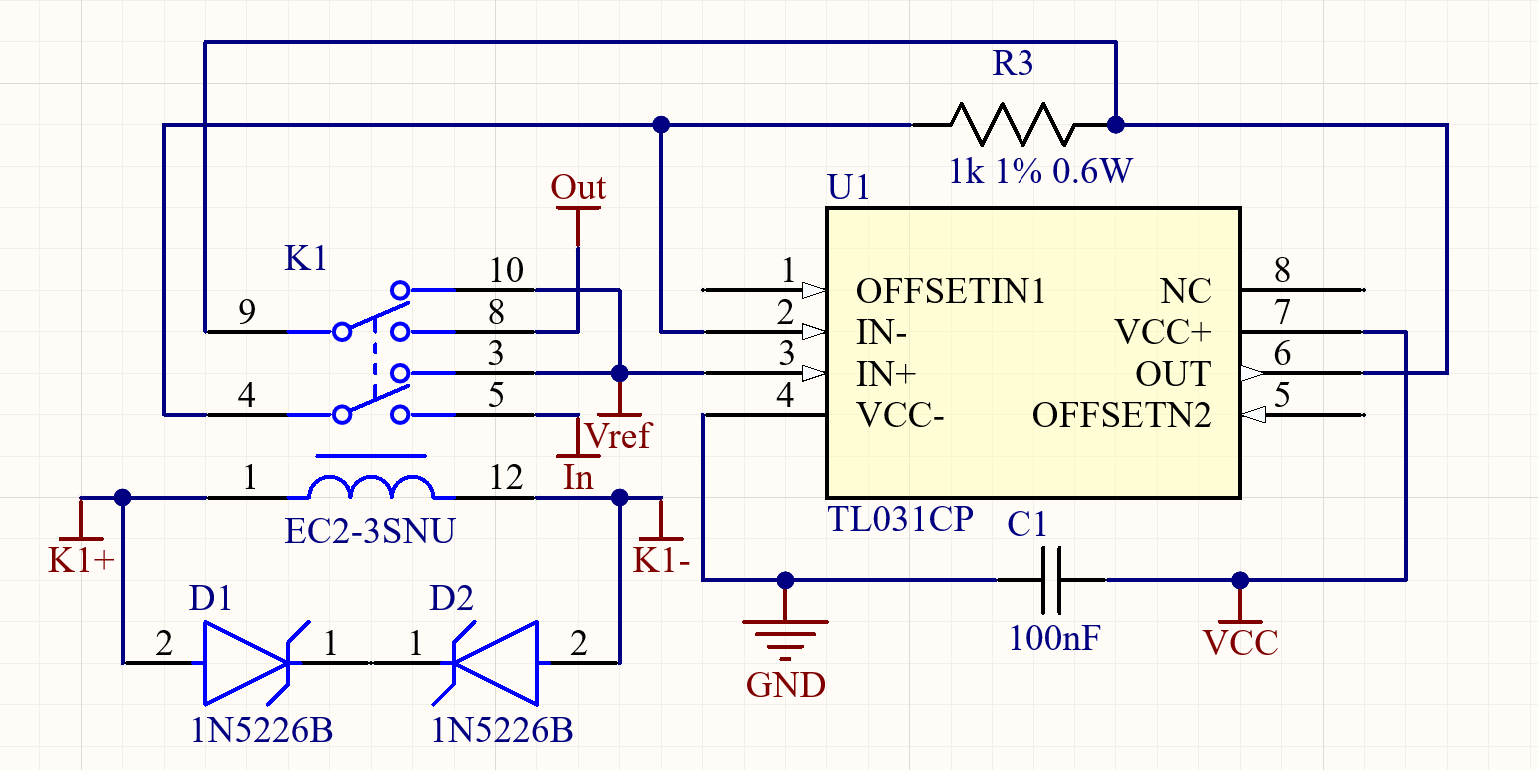
\includegraphics[width=0.8\linewidth]{IndividualTIASchematic.png}
    \caption{Close up of TIA schematic}
    \label{fig:5}
\end{figure}

\subsection{Components}

The bill of materials in figure \ref{fig:6} contains all the components required to manufacture the TIA PCB. All the resistors were chosen for their tolerance to be at or below 1\%. The Zener diodes, which can be seen in figure \ref{fig:7.5}, provide a path for back emf current to flow that prevents damage to the BeagleBone when the latching relays are switched. The op-amps were chosen for their low input bias current (2pA typical at room temperature). 

\begin{figure}
    \centering
    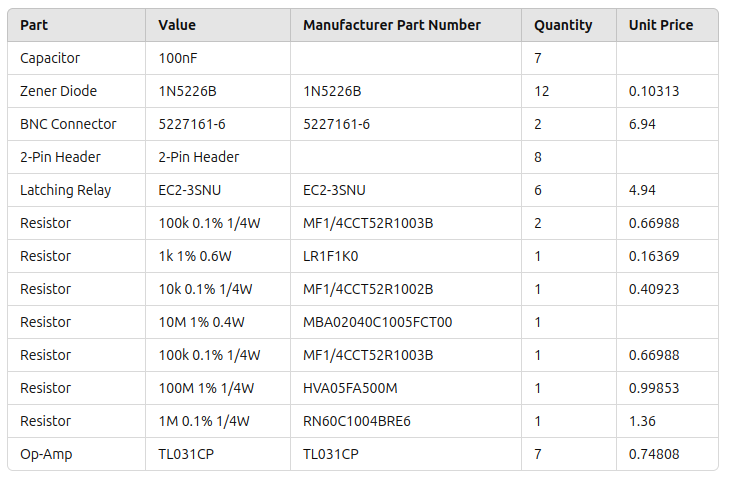
\includegraphics[width=\linewidth]{BOMcropped.png}
    \caption{Bill of Materials for the PCB}
    \label{fig:6}
\end{figure}

\subsection{PCB}

\begin{figure}
    \centering
    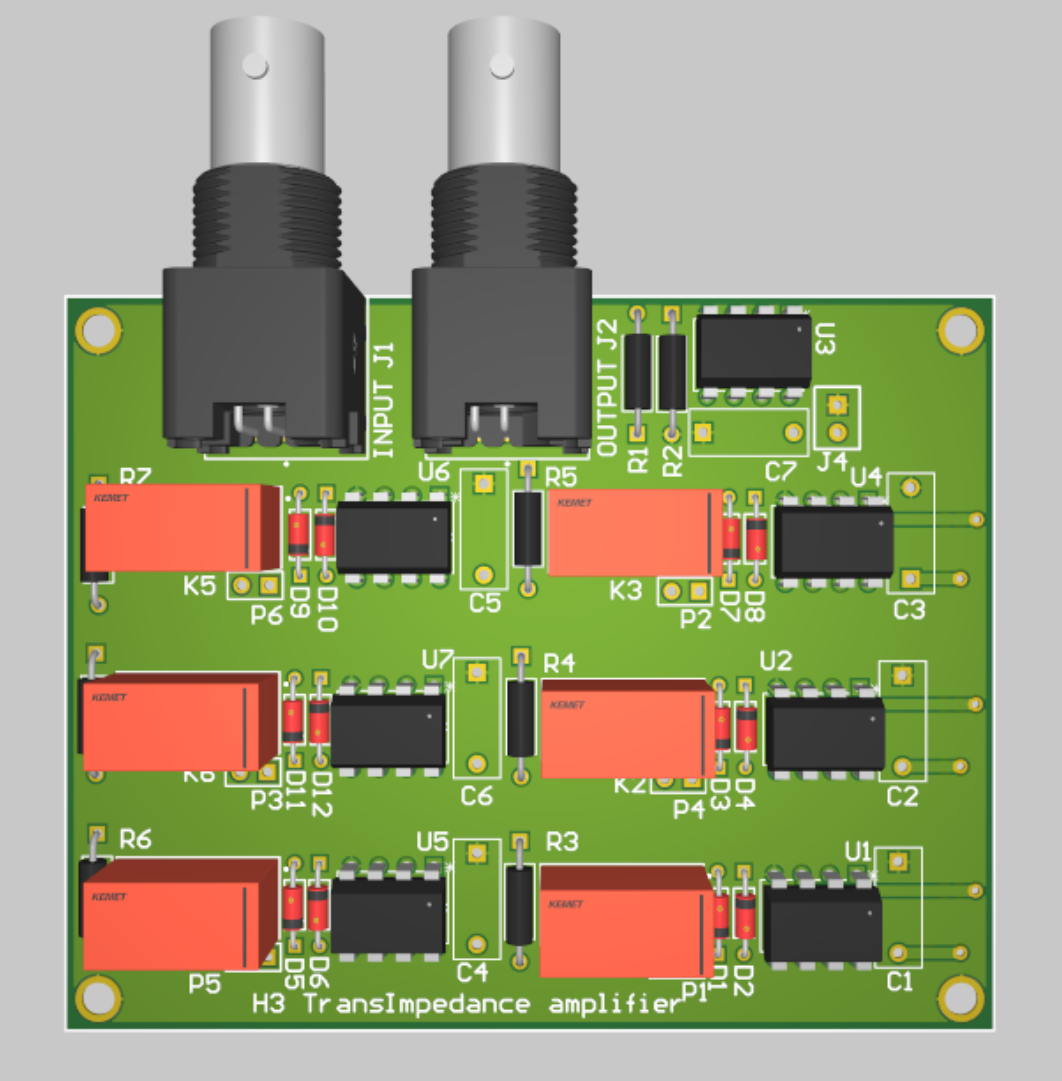
\includegraphics[width=\linewidth]{TIA_PCB_pic.png}
    \caption{TIA PCB}
    \label{fig:7}
\end{figure}

\begin{figure}
    \centering
    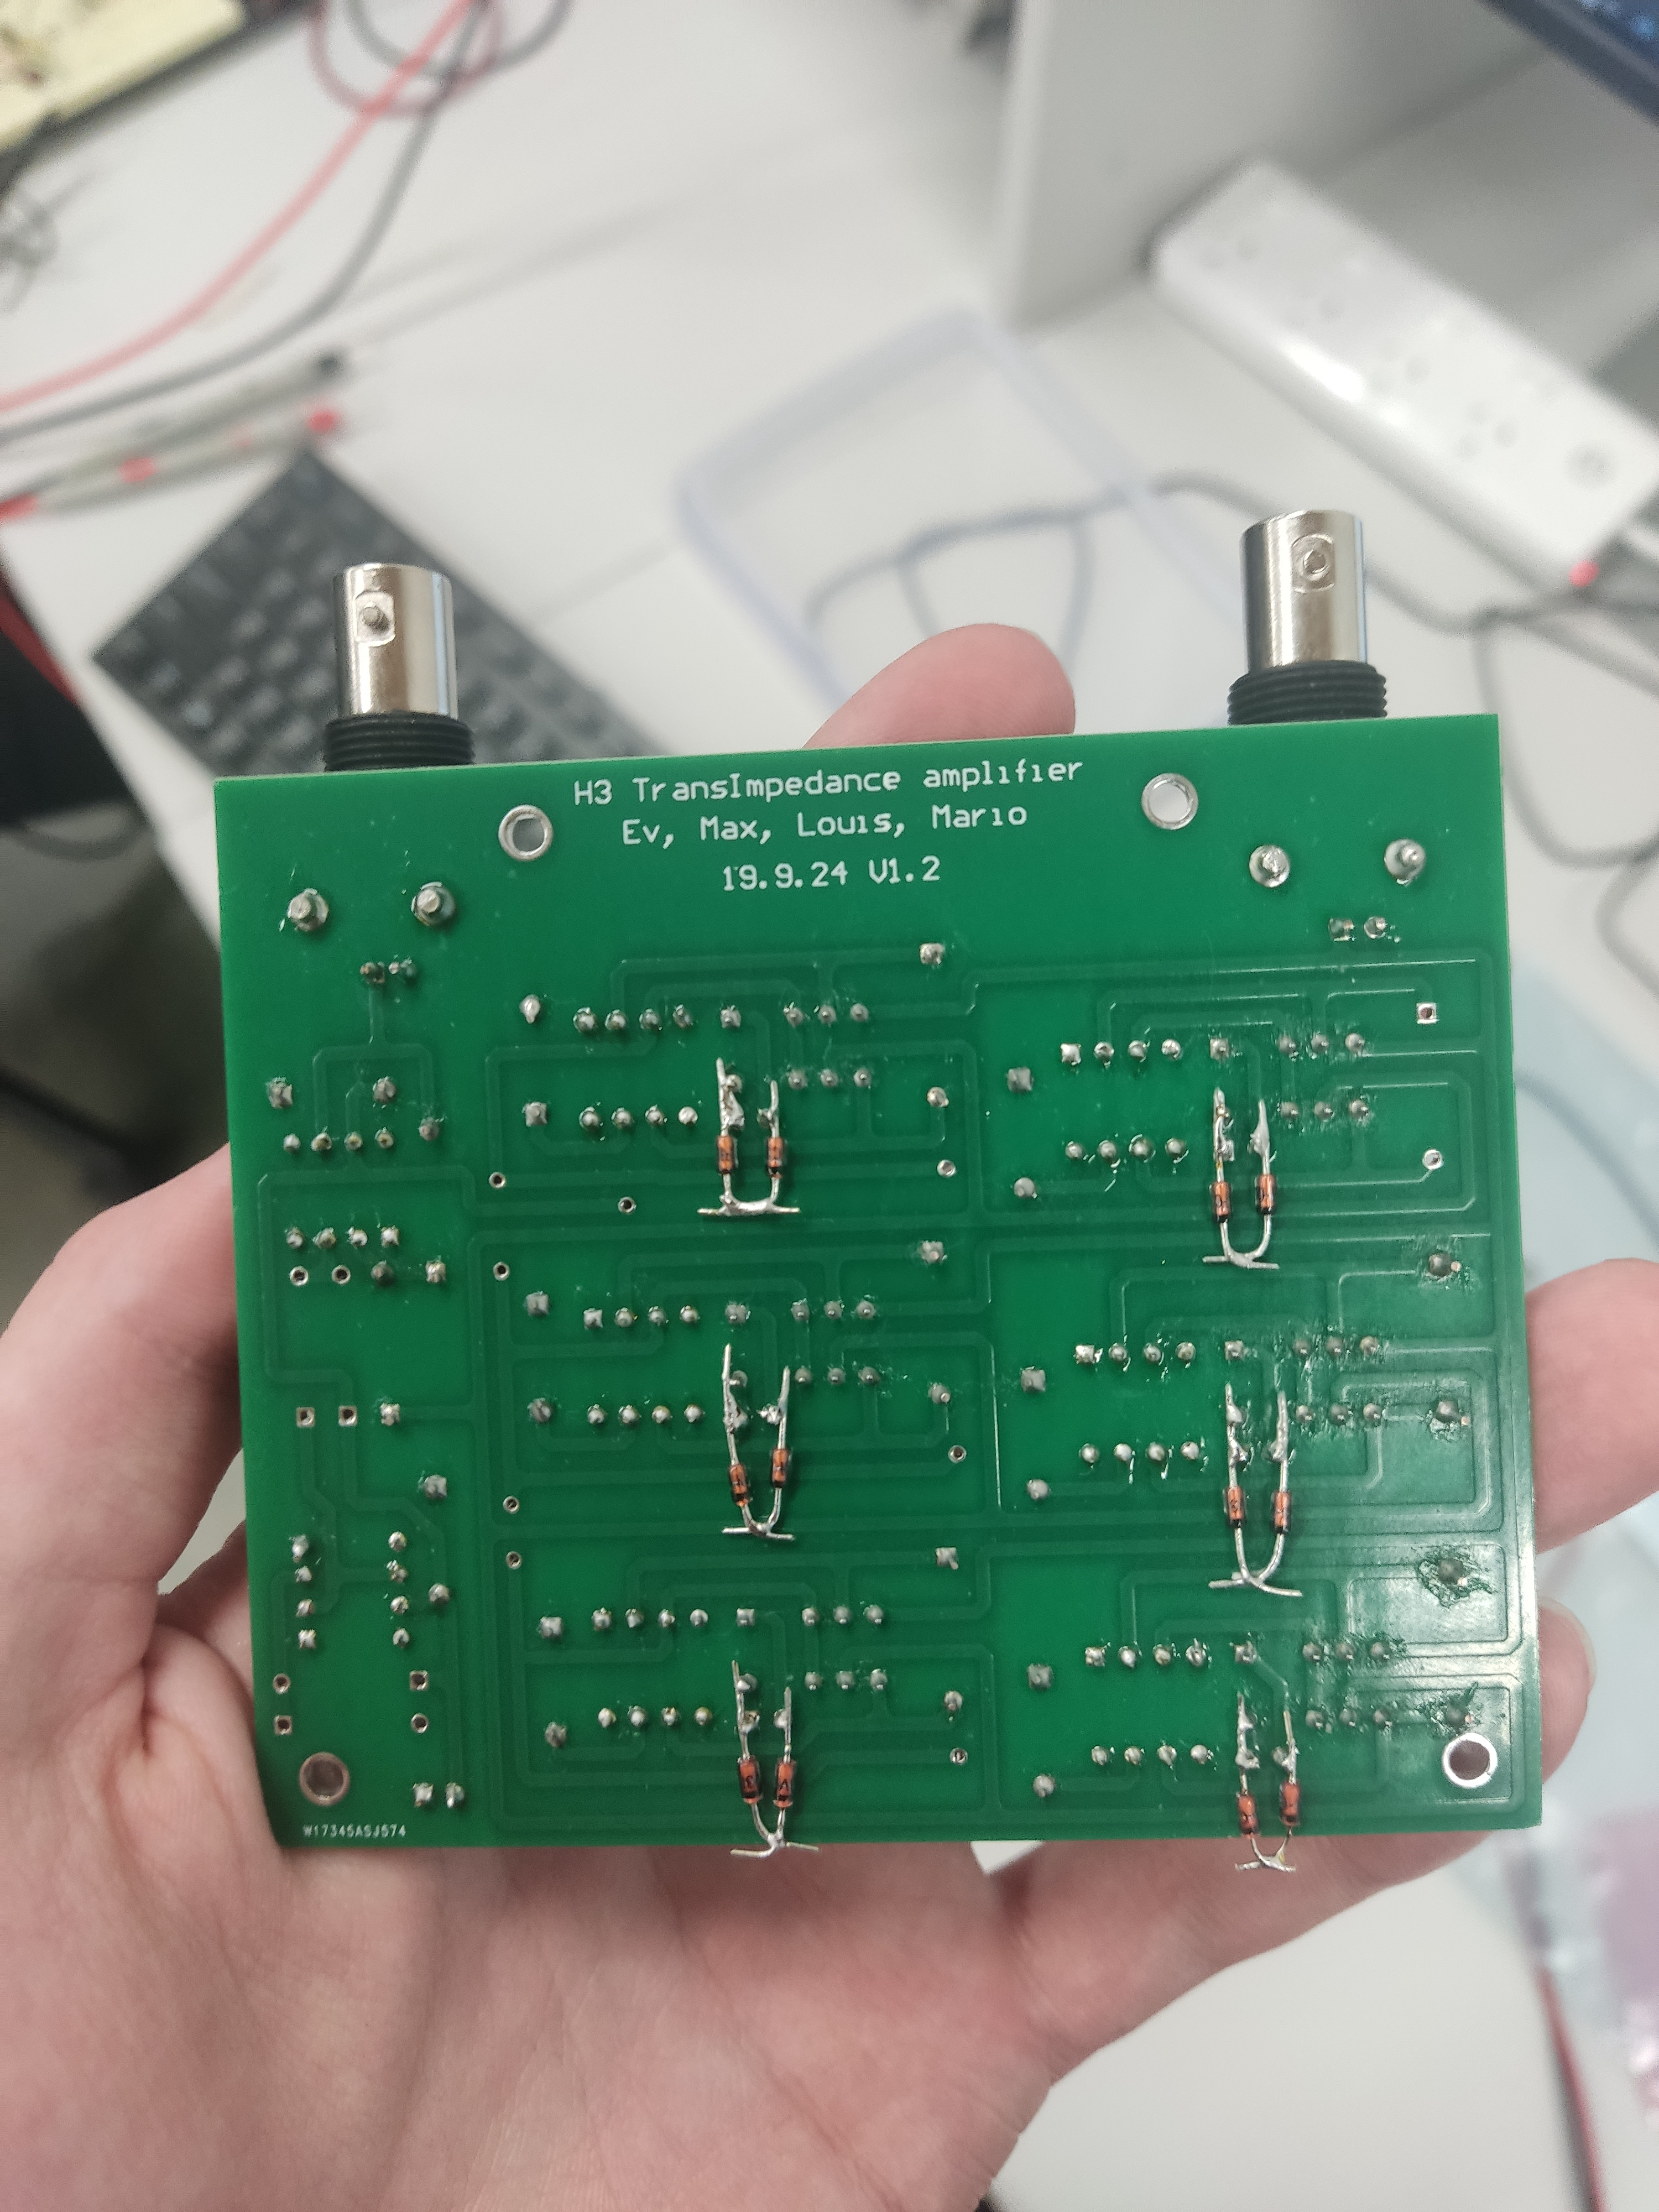
\includegraphics[width=\linewidth]{TIA_PCB_backpic.jpg}
    \caption{Back of the TIA PCB, with Zener diodes}
    \label{fig:7.5}
\end{figure}

\subsection{Software}

The core functionality of the TCP server, running on the BeagleBone, centers around three key processes: managing client connections, interpreting commands, and interacting with the GPIO pins to control the hardware. Each of these processes plays a vital role in ensuring smooth communication between the client and the transimpedance amplifier.\\


\subsubsection{Client Connection Management}

The server starts by creating a socket and binding it to a specific port. It then enters a listening state, where it waits for incoming client connections. Once a connection is established, the server calls a handler to manage that client.\\

The connection management is handled through a blocking event loop to ensure the server remains in the state chosen by a user instead of having modes changed by other users while in use. The main components of this are:\\

\begin{itemize}
    \item Socket Creation and Binding: The server creates a TCP socket using the socket() function, binds it to the specified port, and sets it into listening mode with listen().
    \item Client Handling: When a client connects, the server uses accept() to establish the connection. Following accepting the connection the socket is passed to a handler in message.c to handle communications with the client which initially sends the contents of “welcome.txt” explaining the functionality of the device.
    \item Input Parsing: Upon the client sending a message, the server processes the incoming data character-by-character in a buffer. The server checks for newline characters to detect when a full command is received then converts the message to lower-case to avoid input errors.\\
\end{itemize}


\subsubsection{Command Interpretation and Execution}

Once a command is received from the client, the server proceeds to interpret the command based on its structure. The two primary commands are Gain $<mode\_number>$ and Status, both of which trigger specific functions in the back end.\\

\begin{itemize}
    \item Gain Command: This command switches the gain mode of the transimpedance amplifier. The command parser splits the input string to extract the mode number (e.g. in “Gain 2”, the mode number is 2). Based on the mode number, the server initiates a mode change by activating the appropriate GPIO pins that control the relays for the amplifier. A map of which mode number corresponds to which gain level is provided upon connection to the server and can be accessed again at any time while connected by using the “help” command. Each gain mode is mapped to two specific GPIO pins, and the server interacts with these pins through the following steps:
    \item 1. Deactivate Current Mode: Due to the use of latching relays to deactivate a mode the selection pins required a voltage applied in a certain polarity to turn the relay off. 
    \item 2. Activate New Mode: The opposite polarity voltage was applied to the selection pins to activate a new mode. 
\end{itemize}

A key function in this is the $gpio\_write()$ function found within message.c which controls the high and low states of the GPIO pins by writing directly to the BeagleBone Black’s GPIO file system. Timing between transitions is managed to ensure no incorrect pin states are set during mode changes and the relays have enough time to latch before switching the power off. \\

\begin{itemize}
    \item Status Command: When the server receives a “Status” command, it retrieves the current mode from memory. The server then sends the current mode number back to the client, allowing for real-time feedback for the user. 
    \item Help Command: Typing “help” sends the contents of the “help.txt” file explaining the various servers' various commands.
    \item Exit Command: Disconnects the user from the server.\\
\end{itemize}


\subsubsection{Hardware Control and GPIO Pin Management}
The interaction between the TCP server and the hardware is managed through GPIO pin control, as each gain mode requires the activation of specific GPIO pins. The server uses a structured approach to ensure that the hardware operates reliably:\\

\begin{itemize}
    \item Pin Exporting and Setup: The server first exports the necessary GPIO pins and configures their direction (input/output). During initialization, all pins are set to low to ensure a clean starting state. This is handled by the $gpio\_init()$ function, which ensures that no relays are mistakenly activated when the server starts.
    \item GPIO Initialization: During the server’s startup, a configuration file is loaded using the $load\_configuration()$ function, which defines the GPIO pin assignments for each gain mode. Within this function, all of the relays were powered to ensure that they are all latched in the off state before the user began interacting with it.\\
\end{itemize}


\subsubsection{Error Handling and Robustness}

To ensure that the system operates smoothly, the server incorporates several layers of error handling:\\

\begin{itemize}
    \item Invalid Commands: If a client sends an invalid command (e.g., incorrect mode number), the server responds with an error message and maintains the current hardware configuration. This prevents unwanted changes due to erroneous input.
    \item Connection Stability: The server monitors client connections for timeouts or abrupt disconnections, ensuring that any unresponsive clients are properly handled without affecting future users.\\
\end{itemize}


\subsubsection{Issues and Future work}
At present there appears to be a compiler issue where the program writes pin 0 to each of the GPIO files each time I also write a standard GPIO issue. The server still activates the correct pins but an error is generated each time which has taken some work to handle. \\

In future, the executable generated from this code needs to be pointed to by the “rc.local” file within Linux to allow it to be run when the Beaglebone boots up. Parallel to this, the executable permissions need to be updated to allow a standard user to operate it as socket system commands require “Super User” permissions at present.

\begin{figure}
    \centering
    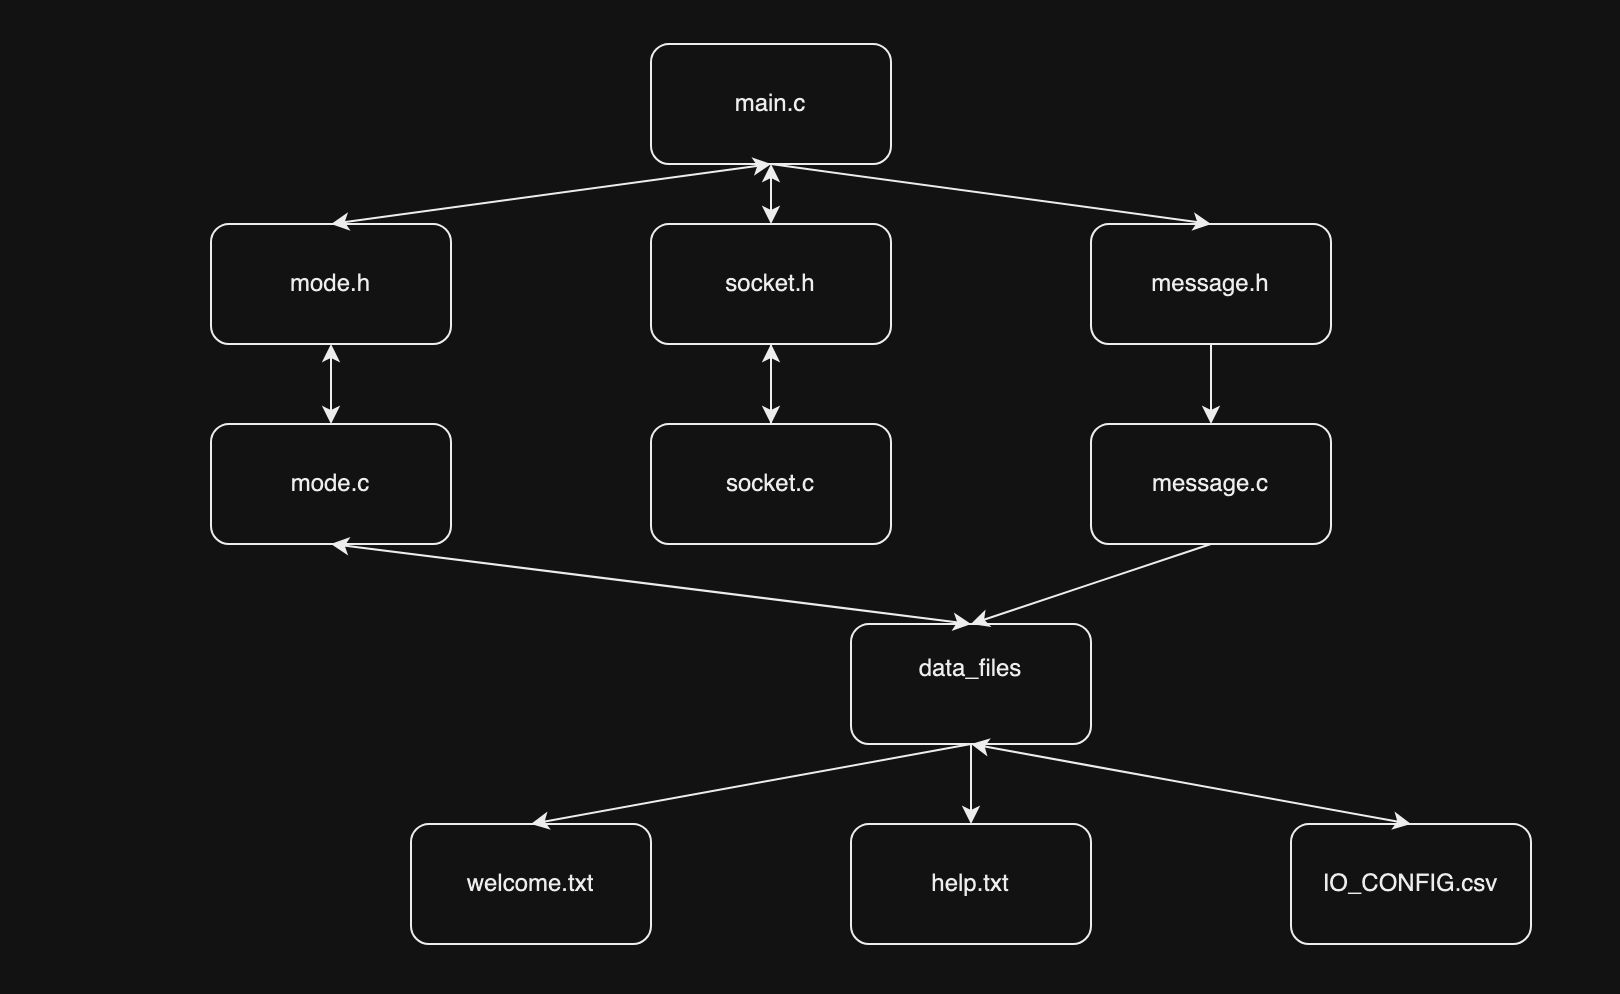
\includegraphics[width=\linewidth]{SoftwareGraph.png}
    \caption{Illustration of the software structure}
    \label{fig:8}
\end{figure}


\section{Evaluation}


The data provided offers insight into the performance of a voltage-controlled current source (VCCS)—a device that produces a current output proportional to a given input voltage—when paired with a transimpedance amplifier (TIA), which converts current into a corresponding output voltage. Several key parameters were measured, including the input voltage, the VCCS current, gain resistor values, and the output voltage. The error between the expected and actual output voltages was calculated to assess the system's overall accuracy and reliability across varying conditions.\\

\subsection{General Observations:}

\begin{enumerate}
    \item \textbf{Low Gain Resistor Values (1 k$\Omega$ and 10 k$\Omega$):}
    \begin{itemize}
        \item For smaller gain resistor values (1 k$\Omega$ and 10 k$\Omega$), the VCCS and TIA demonstrated good agreement between expected and actual output voltages. The errors were minimal, generally less than 1\%, and decreased as the input voltage increased. The stable behaviour of the system in this range indicates that the interaction between the VCCS and TIA is well-controlled, with the VCCS providing accurate currents and the TIA effectively converting those currents to output voltages.\\
    \end{itemize}
    \item \textbf{Intermediate Gain Resistor Values (100 k$\Omega$):}
    \begin{itemize}
        \item At higher gain values, such as 100 k$\Omega$, the system began to show noticeable discrepancies between expected and actual output voltages, particularly at low input voltages. For instance, at 1 V, the error reached -134.33\%. This deviation suggests that the interaction between the VCCS and the TIA becomes problematic as the gain increases.
        \item The inaccuracy at low currents can likely be attributed to the VCCS’s difficulty in delivering precise, stable currents under these conditions. The TIA, in turn, amplifies any small variations or noise in the current, leading to larger errors in the output voltage. While the errors decrease as the input voltage increases, the growing instability at high gain is indicative of challenges in maintaining accurate current control within the VCCS in combination with the high-gain TIA circuit.
    \end{itemize}
    \item \textbf{High Gain Resistor Values (1 M$\Omega$)}
    \begin{itemize}
        \item When the gain resistor was increased to 1 M$\Omega$, significant deviations were observed across the entire voltage range. The errors were particularly large at low voltages, with a -250.2\% error at 1 V. These results suggest that the VCCS struggles to deliver the very small currents required for high-gain configurations, leading to substantial inaccuracies when interacting with the TIA.
        \item The TIA’s amplification of the small, inaccurate current signals produced by the VCCS under high-gain conditions magnifies these errors further. Noise and offset variations from the VCCS are amplified in the TIA circuit, resulting in significant deviations in the output voltage. This behaviour highlights the limitations of the VCCS in providing accurate, low-level currents when paired with a high-gain TIA.\\
    \end{itemize}
\end{enumerate}

\subsection{Error Analysis:}

\begin{itemize}
    \item \textbf{Smaller Errors at Low Gain:} For 1 k$\Omega$ and 10 k$\Omega$ resistors, the VCCS and TIA interact effectively, with low errors suggesting accurate current delivery and minimal amplification of noise.
    \item \textbf{Increased Errors at High Gain:} At 100 k$\Omega$ and 1 M$\Omega$, errors increase dramatically due to the VCCS’s inability to deliver precise small currents, which is then magnified by the TIA, leading to significant inaccuracies in the system output.\\
\end{itemize}


\subsection{Potential Causes of Error:}

\begin{itemize}
    \item \textbf{Current Instability from the VCCS:} The VCCS struggles to provide accurate, low-level currents, particularly at high gain resistor settings. This leads to increased noise and variations in the current, which the TIA amplifies, resulting in large output voltage errors.
    \item \textbf{Amplified Noise:} The TIA amplifies not only the current but also any imperfections or noise in the current provided by the VCCS. At high gain settings, this noise becomes significant, contributing to the observed output discrepancies.\\
\end{itemize}


\textbf{Impact of Testing with a 10 M$\Omega$ Gain Resistor:} Testing with a 10 M$\Omega$ gain resistor was not conducted, but it can be reasonably predicted that the interaction between the VCCS and TIA would have led to even greater instability and larger errors. At such high gain, the VCCS would struggle even more to provide the extremely low and stable currents required, resulting in significant inaccuracies in the output voltage due to amplified noise and signal instability. Errors could be expected to exceed those observed with the 1 M$\Omega$ resistor, further emphasising the limitations of the VCCS in this high-gain configuration.\\

\textbf{Results:} The system performs well for lower gain resistor values (1 k$\Omega$ and 10 k$\Omega$), where the VCCS and TIA interact with minimal error. However, as the gain increases, the VCCS’s inability to provide accurate low currents becomes more pronounced, leading to significant errors when interacting with the TIA. At high gain settings (100 k$\Omega$, 1 M$\Omega$), the VCCS’s current inaccuracies are magnified by the TIA, resulting in large deviations between expected and actual output voltages. Testing with a 10 M$\Omega$ resistor would likely exacerbate these issues, further highlighting the limitations of the VCCS in maintaining precise current control in high-gain scenarios.

\begin{figure}
    \centering
    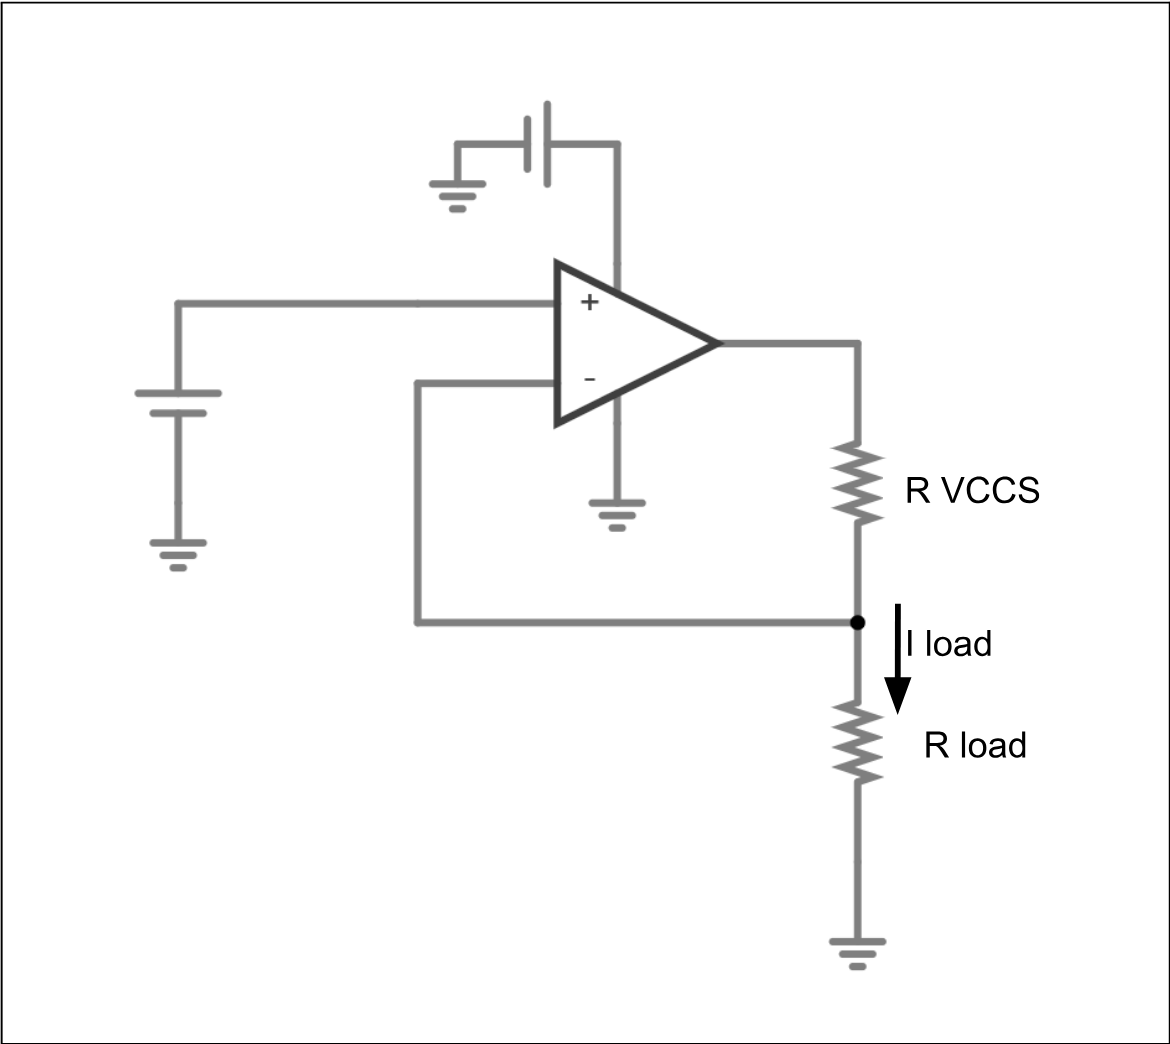
\includegraphics[width=\linewidth]{VCCS_schematic.png}
    \caption{Basic Schematic of a VCCS}
    \label{fig:9}
\end{figure}

\begin{figure}
    \centering
    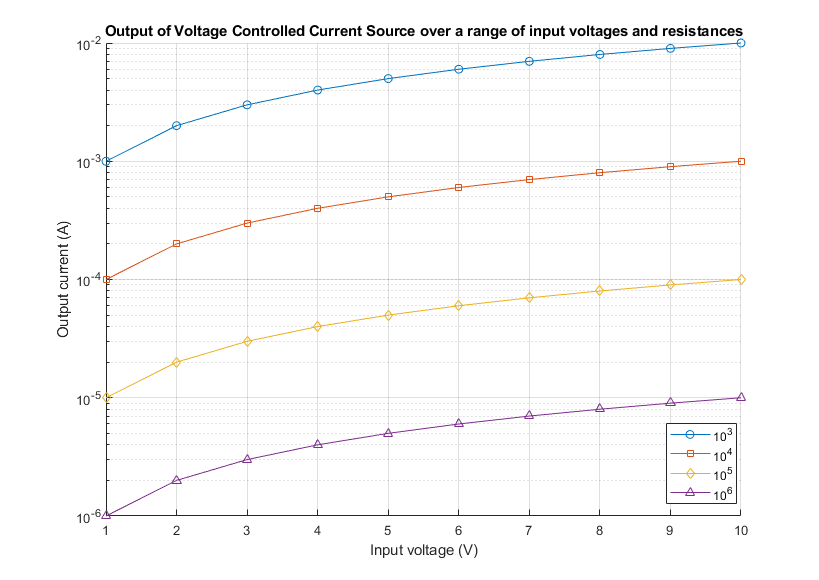
\includegraphics[width=\linewidth]{VCCSplot.png}
    \caption{voltage current graph of VCCS}
    \label{fig:10}
\end{figure}

\begin{figure}
    \centering
    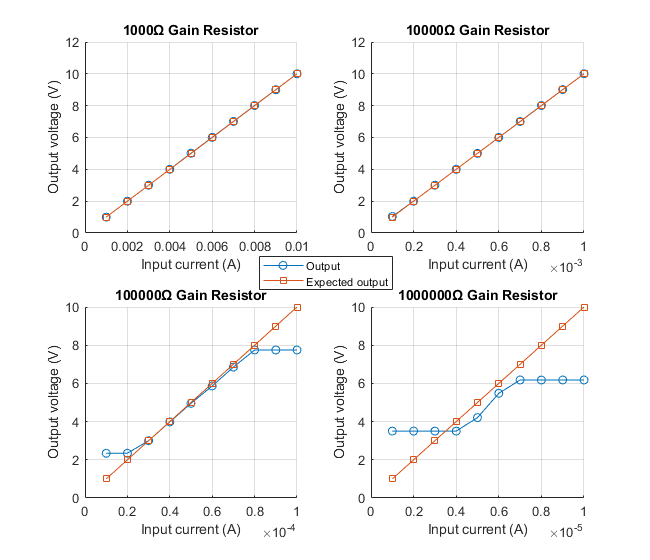
\includegraphics[width=\linewidth]{TIA_VvsI.png}
    \caption{Output Voltage over input Current of TIA tests}
    \label{fig:11}
\end{figure}

\begin{figure}
    \centering
    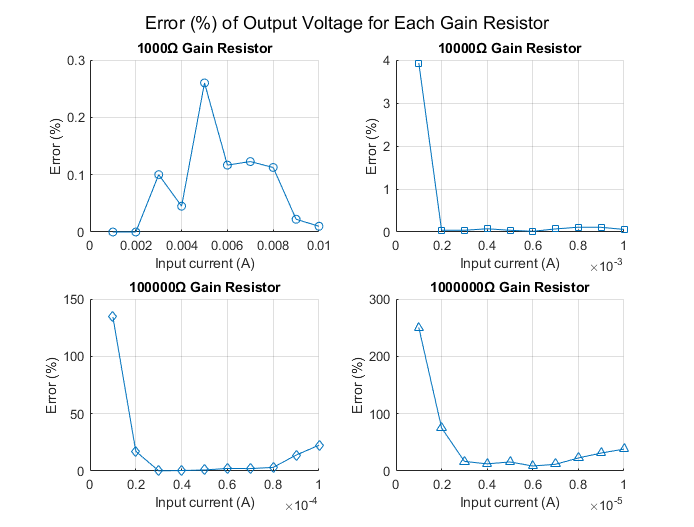
\includegraphics[width=\linewidth]{TIA_Error.png}
    \caption{Percent error of TIA outputs}
    \label{fig:12}
\end{figure}

\textit{Still need: Additional evaluation results that include the software. to reference the requirements ideally.}




\section{Conclusions \& Future Work}

\textit{Future work should not just be a list of things that you would have done if you had a little more time. Talk about new things that are possible now that you have finished your project. What projects could a ’489 student tackle next year if they started on their '489 project next year from your end point? HINT: This might be a possibility!} \\






% *** REFERENCES ***
\bibliographystyle{IEEEtran}
\bibliography{references}

\end{document}

